\documentclass{ctexart}
\usepackage[left=2.5cm, right=2.5cm, top=1.5cm, bottom=2.5cm]{geometry}
\usepackage{pgf, tikz}
\usepackage{forest}
\usepackage{listings}
\usepackage{amsfonts}
\usepackage{graphics}
\CTEXsetup[format=\Large\bfseries]{section}

\title{\center \rule{16.4cm}{1mm} \\ \rule{3.2cm}{1mm}\hfill \bfseries\Huge socket应用编程实验 \hfill \rule{3.2cm}{1mm}}
\author{\bfseries\Large 熊子威 \\ 2015K8009915050}
\date{}
\begin{document}
\maketitle
\begin{center}
\rule{16.6cm}{0.3mm}  
\end{center}

\section{实验内容}
本实验目标是构建一个基于socket的分布式字符统计程序并在mininet中运行这个程序。程序分为master和worker两个部分。master通过socket接口向两个worker分发任务(需要统计字符数的文件路径,该文件中那个部分需要当前worker去统计),而两个worker则通过socket接口接受来自master的任务分配然后进行字母数目的统计,统计完毕后将二十六个字母的数目再各自发回给master,然后master将两者的统计数据加和并打印出来。
\section{实验流程}
因为第一次使用socket并进行网络编程,对各个API的工作方式不是很了解,因此写代码时是一边测试一边迭代进行的。\par
首先编写一个简单的master和worker,确保master能够和一个worker连接上,然后这个worker发送一条打招呼信息,然后让worker将这条信息打印出来。\par
然后修改这个程序,添加多线程,让master同时和两个worker打招呼,确认listen()这个接口是否只需要主线程监听即可。结果是只需要主线程监听,两个工作线程负责accept然后处理数据传输和处理即可。\par
然后修改这个程序,让master按照顺序分别向两个worker发送两条消息,确认socket对消息发送和接受的顺序是如何处理的。然后发现send和recv是匹配在一起不会发生乱序之后,进一步修改程序。\par
这一步的修改是为mastert添加计算文件总长度并依据worker的不同地址而分别分配不同的任务并且让worker打印出分配来顺便检查工作分配是否正确(文件名是否正确接受,文本划分的起止位置是否正确)。\par
这一步确保能够正确工作之后为worker添加字符统计的代码,并分别打印结果来确认统计结果正确。\par
最后一步为master和worker分别添加接收统计结果和发送统计结果的代码,并为master添加汇总结果的代码。\par
全部完成并却运转正确,和老师的reference输出一致之后,重新修改了master代码的结构,将一些复杂冗长的操作用函数封装,提高代码的可读性。

\section{实验结果}
\noindent 起始阶段:\par
\noindent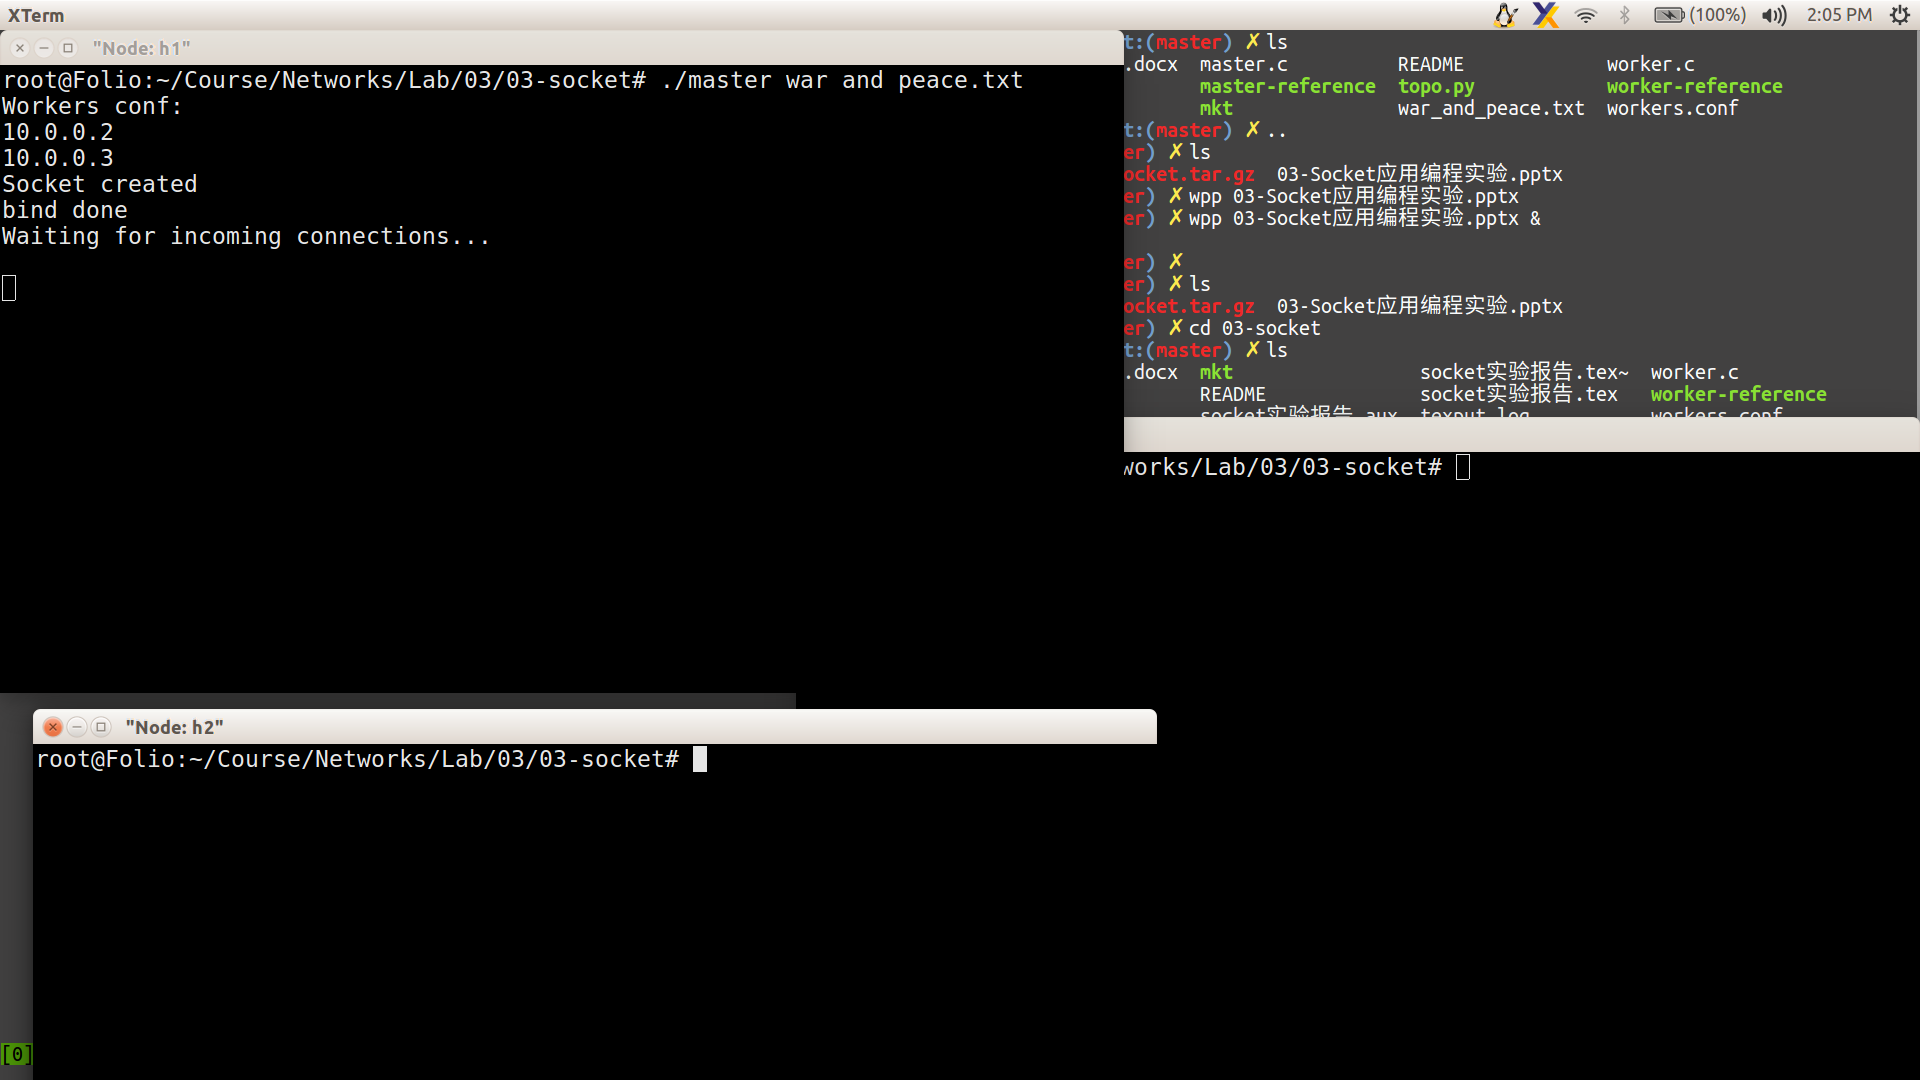
\includegraphics[scale=0.25]{master_worker.png}\\
执行结束:\par
\noindent\includegraphics[scale=0.25]{master_worker_result.png}\\
\noindent 可以看到两个worker成功并且正确地向master发送了相关的数据,而master也成功接受并且完成了最后的结果汇总。
\section{结果分析}
\noindent 可以从master的主要代码来分析\par
\noindent\includegraphics[scale=0.35]{master_main.png}
\includegraphics[scale=0.35]{master_work.png}\\
\noindent master进行了几个阶段的确认,建立server时,分配任务时,确认任务分发成功时,最后获得结果时,都需要确认成功才能进行下一步。相应的,worker也需要进行响应。因此最后的结果如下图所示:\\\par
\noindent\includegraphics[scale=0.27]{worker_1.png} 
\end{document}
